\xchapter{Meu Possante}{}
\label{meupossante}
Mecânica automotiva é um assunto extremamente complexo. Cada um dos inúmeros componentes
do automóvel tem seu próprio ciclo de vida e devem ser revisados e trocados em seu próprio
tempo. Além disso, certas condições de uso podem diminuir a vida útil de algumas peças,
tornando mais frequente a necessidade de revisão.

A falta de conhecimento destes fatos pode levar ao dono de um automóvel negligenciar
as manutenções no tempo correto, causando desde transtornos que poderiam ser facilmente
evitados a acidentes ocasionados por falhas mecânicas.

Em 2016, mais de 2 milhões de automóveis foram vendidos no Brasil
\cite{fenabrave}. Dentre este número, é seguro assumir que poucos de seus
proprietários são especialistas em mecânica e possuem dúvidas sobre o
funcionamento das peças do seu veículo, além de não saber exatamente em qual
momento deve-se trocar cada uma de suas peças. Estas informações geralmente
estão no manual do veículo, mas é inviável para uma pessoa leiga memorizar
todas estas informações.

Após a compra de um automóvel, a sua manutenção é de inteira responsabilidade
do proprietário. Todas as operações de manutenção, especificadas pelo fabricante,
devem ser realizadas dentro dos intervalos apropriados \cite{manualhyundai}.
Proporcionar manutenção apropriada para o veículo, não somente reduz os custos
operacionais, mas também ajuda a impedir mau funcionamento devido a negligência,
caso que geralmente não é coberto por garantia \cite{manualonix}.

Para executar a manutenção apropriadamente, o proprietário precisa estar
sempre atento ao momento correto da troca das peças, que muda de acordo
com as condições de uso de um carro. Acompanhar estas diferentes variáveis pode
ser difícil para pessoas comuns.

O uso de um aplicativo para celular pode ser uma grande ajuda na decisão de quando
é necessário a revisão e troca de peças, alertando o usuário visualmente quando alguma
manutenção está próxima. Neste sentido surge o Meu Possante, um aplicativo que monitora
o estado atual do veículo e avisa o momento em que as manutenções das peças serão
necessárias.

\section{Arquitetura}
\label{meupossante-app}

O Meu Possante possui um objetivo simples: Auxiliar o motorista a identificar quais
peças de seu carro precisarão de manutenção em um futuro próximo. O aplicativo nasceu
como trabalho final da disciplina de Desenvolvimento de Aplicações para Dispositivos
Móveis e está em processo refinamento para publicação na Google Play Store.

A tela principal do aplicativo mostra todos os componentes do veículo que são monitorados,
como pode ser visto na figura \ref{meu-possante-tela-principal}. Ao clicar em um componente,
a tela do mesmo é mostrada, com informações como a frequência de troca e quilometragem
atual.

\begin{figure}[h]
\centering
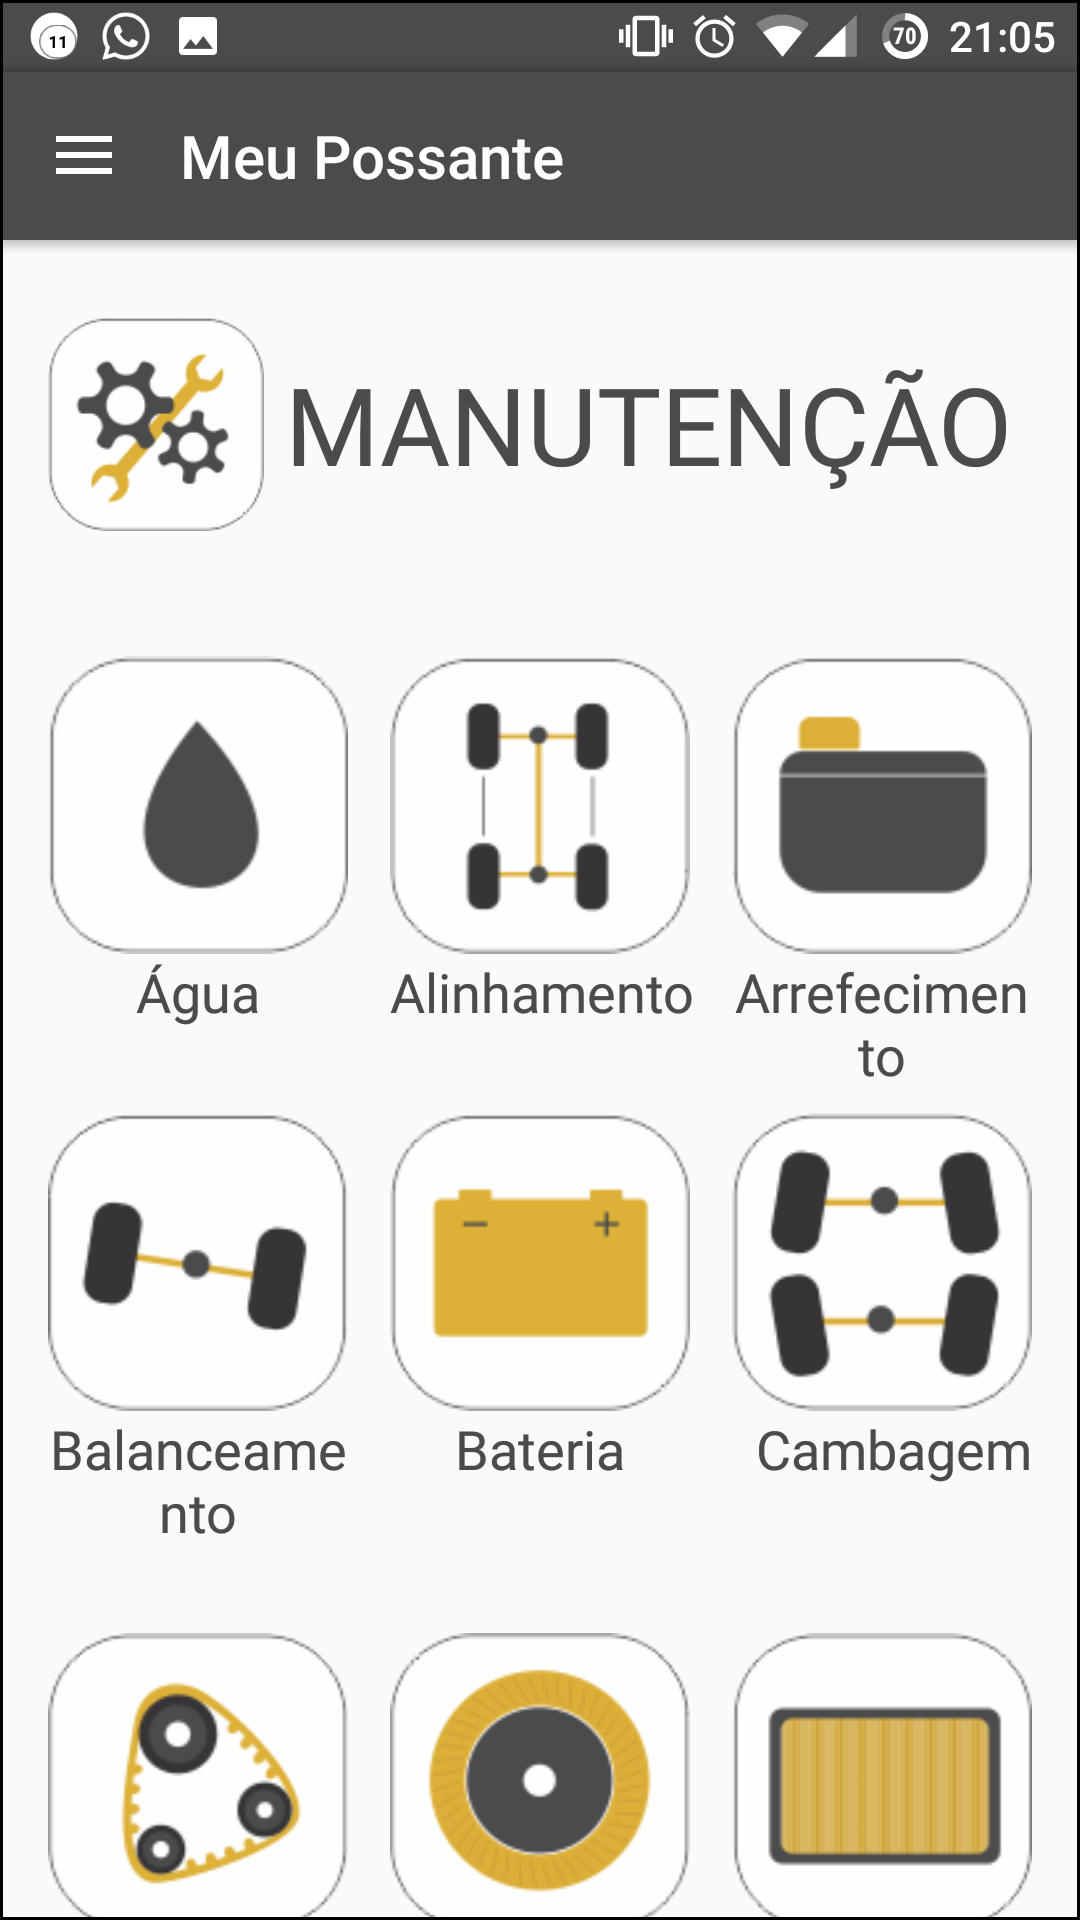
\includegraphics[width=0.3\textwidth]{images/meu-possante-tela-principal.png}
\caption{Tela principal do Meu Possante}
\label{meu-possante-tela-principal}
\end{figure}

O aplicativo utiliza informações do GPS do dispositivo para calcular a distância percorrida
pelo motorista enquanto está dirigindo. No momento em que detecta a iminência de manutenção
de alguma das peças do veículo, uma notificação é enviada para o dispositivo do usuário.
Esta notificação leva à página da peça correspondente no aplicativo, onde pode ser lido
mais detalhes sobre o estado atual, como a quilometragem e qual a quilometragem da
próxima troca, como pode ser visto na figura \ref{meu-possante-tela-componente}.

\begin{figure}[h]
\centering
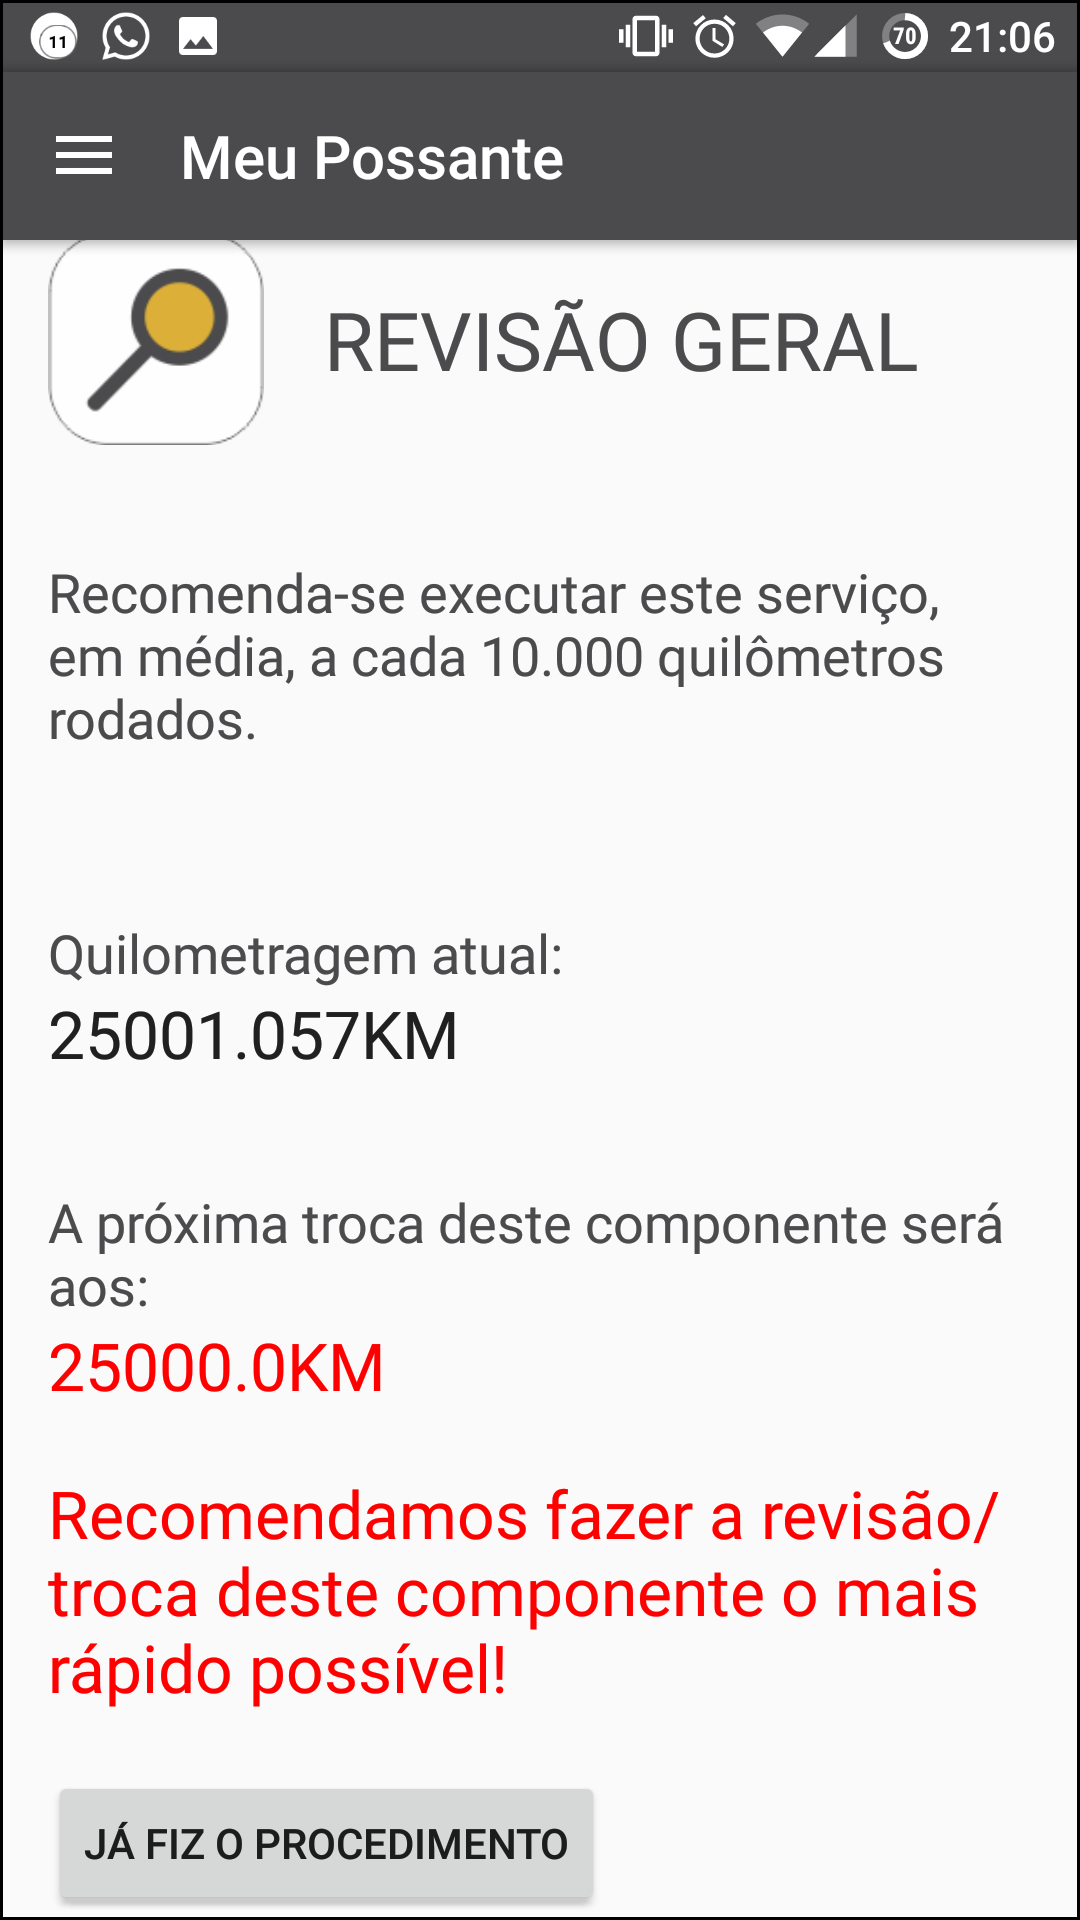
\includegraphics[width=0.3\textwidth]{images/meu-possante-tela-componente.png}
\caption{Tela que indica a necessidade de revisão de um componente}
\label{meu-possante-tela-componente}
\end{figure}

Um exemplo do caso supracitado é o fluido de freio, cuja troca recomendada é a cada
10.000 quilômetros rodados ou 1 ano, o que ocorrer primeiro. Já a troca da correia
dentada deve ser feita a cada 50.000 quilômetros, sem limite de tempo definido. Os
outros componentes funcionam da mesma forma, cada qual com sua quilometragem e
tempo de troca específicos.

Na versão atual, o motorista precisa indicar que está dirigindo através de uma tela
específica. Ao indicar que está dirigindo, o aplicativo começa a monitorar a localização
do usuário e seu deslocamento. Durante a corrida, os dados de quilometragem são atualizados
no banco de dados e na iminência da manutenção de uma peça, uma notificação é enviada para o
usuário.

O Meu Possante foi pensado de forma a ter uma arquitetura simples e eficiente. Na figura
é possível ver o fluxo de dados através dos módulos, começando pela entrada de dados do GPS
e chegando ao final com a atualização destes dados em um banco de dados e o eventual envio de
uma notificação. As setas na imagem indicam o sentido do fluxo de dados.

\begin{figure}[h]
  \centering
  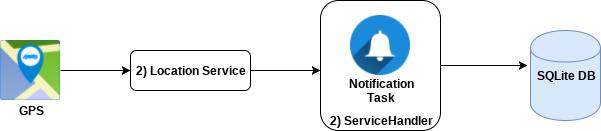
\includegraphics[width=0.7\textwidth]{images/arquitetura-meu-possante.png}
  \caption{Arquitetura do Meu Possante}
  \label{meu-possante-arquitetura}
\end{figure}

Os módulos utilizados são os seguintes:

\begin{enumerate}
  \item \textbf{Location Service:} Responsável pela configuração e gerenciamento do sensor de localização (GPS).
    O monitoramento do sensor é feito através de um serviço que continua rodando no background,
    mesmo quando o usuário não está com a aplicação aberta.
  \item \textbf{Service Handler:} Responsável pela inicialização e checagem de dados dos serviços
    que estão rodando na aplicação. Este módulo também é responsável por atualizar as informações
    de quilometragem no banco de dados e notificar o usuário, caso detecte a iminência de
    manutenção de alguma peça.
\end{enumerate}

A solução proposta no presente trabalho almeja estender o módulo Service Handler para que não notifique motoristas
em momentos inoportunos, evitando colocá-los em potenciais riscos. O próximo capítulo explica com mais detalhes
o porquê da notificação de motoristas em momentos inoportunos ser um problema.
